\section{Phân phối Gamma (Gamma Distribution)}
	Phân phối Gamma là một phân phối xác suất liên tục, dương và có hình dạng linh hoạt, thường được sử dụng để mô hình hóa thời gian chờ đợi hoặc các đại lượng dương có tính chất kéo dài.
	
	\subsection{Định nghĩa}
	
	Một biến ngẫu nhiên $X$ tuân theo phân phối Gamma với tham số hình dạng (shape parameter) $k > 0$ và tham số tỷ lệ (scale parameter) $\theta > 0$, ký hiệu $X \sim \text{Gamma}(k, \theta)$, có hàm mật độ xác suất (PDF) được cho bởi:
	\[ f(x; k, \theta) = \frac{x^{k-1} e^{-x/\theta}}{\Gamma(k) \theta^k} \quad \text{với } x > 0 \]
	Trong đó, $\Gamma(k)$ là hàm Gamma, được định nghĩa là $\Gamma(k) = \int_0^\infty t^{k-1} e^{-t} dt$.
	
	\subsection{Hàm xác suất tích lũy (Cumulative Distribution Function - CDF)}
	Hàm xác suất tích lũy của phân phối Gamma không có dạng đóng (closed-form) đơn giản và thường được biểu diễn thông qua hàm Gamma không đầy đủ quy chuẩn (regularized lower incomplete gamma function) $P(k, x/\theta)$:
	\[ F(x; k, \theta) = P\left(k, \frac{x}{\theta}\right) = \frac{1}{\Gamma(k)} \int_0^x t^{k-1} e^{-t/\theta} dt \]
	
	\subsection{Các đặc trưng thống kê}
	\begin{itemize}
		\item \textbf{Miền giá trị:} $x \in (0, \infty)$.
		\item \textbf{Giá trị kỳ vọng (Mean):} $E[X] = k\theta$.
		\item \textbf{Phương sai (Variance):} $\text{Var}[X] = k\theta^2$.
		\item \textbf{Mode:}
		\[ \text{Mode} = \begin{cases} (k-1)\theta & \text{nếu } k > 1 \\ \text{không xác định (tại 0)} & \text{nếu } k \le 1 \end{cases} \]
		\item \textbf{Median:} Không có dạng đóng. Đối với các giá trị lớn của $k$, median xấp xỉ $k\theta - \frac{1}{3}\theta$.
		\item \textbf{Tính chất đối xứng/lệch:}
		Phân phối Gamma thường bị lệch phải. Khi $k$ tăng, phân phối trở nên đối xứng hơn. Hệ số lệch (skewness) là $\frac{2}{\sqrt{k}}$.
	\end{itemize}
	
	\subsection{Biểu đồ minh họa}
	Dưới đây là biểu đồ minh họa hàm mật độ xác suất 
	và hàm xác suất tích lũy của phân phối Gamma với các giá trị khác nhau của tham số hình dạng 
	$k$ và tham số tỷ lệ $\theta$.
	
	\begin{figure}[h!]
		\centering
		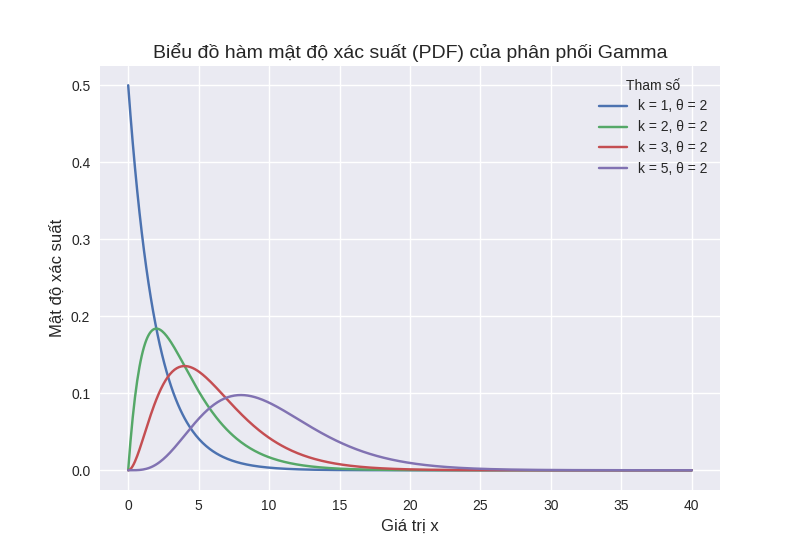
\includegraphics[width=0.5\textwidth]{images/Gamma Distribution-PDF.png} % Placeholder cho hình ảnh
		\caption{Hàm mật độ xác suất của Phân phối Gamma với các tham số khác nhau.}
		\label{fig:Gamma Distribution-PDF}
	\end{figure}
	\begin{figure}[h!]
		\centering
		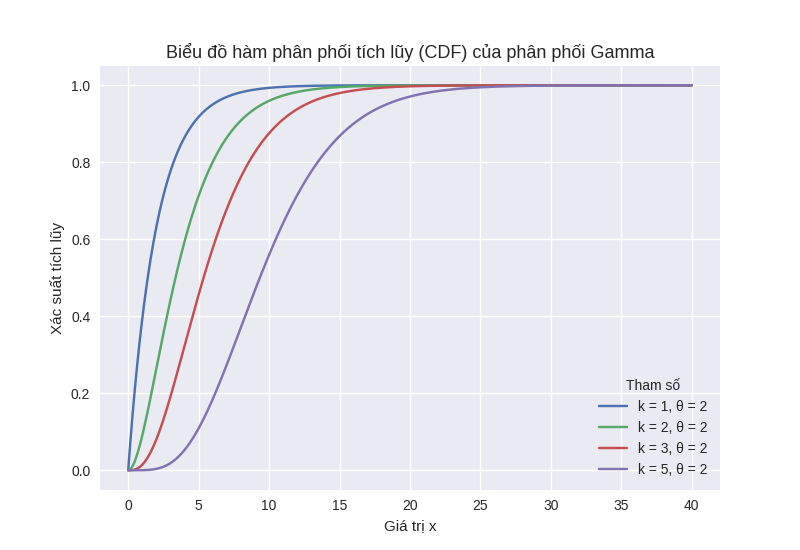
\includegraphics[width=0.5\textwidth]{images/Gamma Distribution-CDF.png} % Placeholder cho hình ảnh
		\caption{Hàm mật độ xác suất của Phân phối Gamma với các tham số khác nhau.}
		\label{fig:Gamma Distribution-CDF}
	\end{figure}
	

	\newpage
	\subsection{Ví dụ dữ liệu và bài toán thực tế}

	Giả sử ta đang phân tích thời gian giữa các cuộc gọi đến tổng đài:

	\begin{center}
	\begin{tabular}{|c|c|}
	\hline
	Cuộc gọi thứ & Thời gian giữa các cuộc gọi (phút) \\
	\hline
	1 & 3.2 \\
	2 & 5.1 \\
	3 & 2.7 \\
	4 & 4.3 \\
	5 & 6.0 \\
	\hline
	\end{tabular}
	\end{center}

	Ta giả sử thời gian giữa các cuộc gọi tuân theo phân phối Gamma:

	\[
	X \sim \text{Gamma}(\alpha, \beta)
	\]

	Phân phối Gamma có mật độ xác suất:

	\[
	f(x; \alpha, \beta) = \frac{\beta^\alpha}{\Gamma(\alpha)} x^{\alpha - 1} e^{-\beta x}, \quad x > 0
	\]

	Phân phối này giúp mô hình hóa thời gian giữa các sự kiện ngẫu nhiên một cách linh hoạt và hiệu quả.
	\begin{figure}[h!]
		\centering
		
		% Minipage cho hình ảnh thứ nhất (Cột 1)
		\begin{subfigure}[b]{0.49\textwidth}
			\centering
			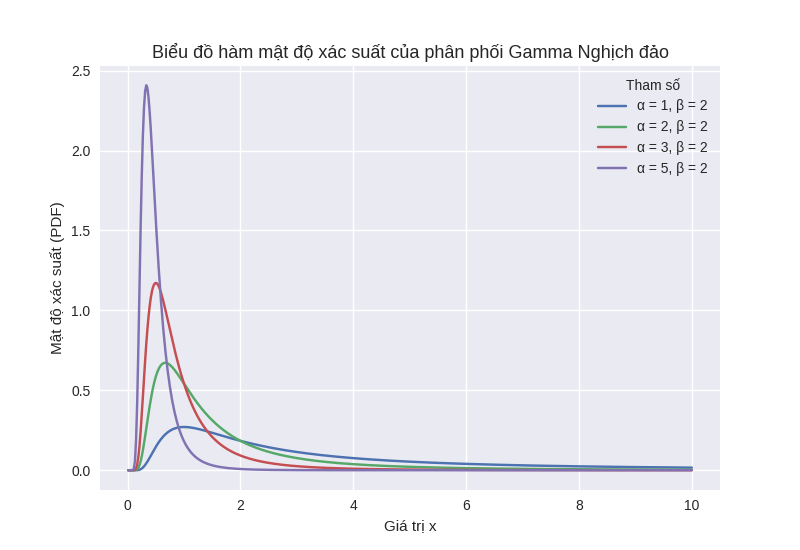
\includegraphics[width=\textwidth]{images/Inverse Gamma Distribution-PDF.png}
			\caption{Hàm mật độ xác suất (PDF).}
			\label{fig:InverseGamma-PDF}
		\end{subfigure}
		% Khoảng cách giữa hai cột (có thể dùng \hfill nếu muốn căn lề hoàn toàn)
		\hfill 
		% Minipage cho hình ảnh thứ hai (Cột 2)
		\begin{subfigure}[b]{0.49\textwidth}
			\centering
			\includegraphics[width=\textwidth]{images/Inverse Gamma Distribution-CDF.png}
			\caption{Hàm xác suất tích lũy (CDF).}
			\label{fig:InverseGamma-CDF}
		\end{subfigure}
		
		% Chú thích chung cho cả hai hình
		\caption{So sánh Hàm mật độ xác suất và Hàm xác suất tích lũy của Phân phối Gamma Nghịch đảo (Inverse Gamma Distribution) với các tham số khác nhau.}
		\label{fig:InverseGamma-Combined}
	\end{figure}
\newpage
\section{Phân phối Beta (Beta Distribution)}
	Phân phối Beta là một phân phối xác suất liên tục được định nghĩa trên khoảng $[0, 1]$. Nó rất hữu ích để mô hình hóa các đại lượng có giá trị giới hạn trong khoảng này, chẳng hạn như xác suất, tỷ lệ hoặc tỷ lệ phần trăm.
	
	
	\subsection{Định nghĩa}
		Một biến ngẫu nhiên $X$ tuân theo phân phối Beta với hai tham số hình dạng $\alpha > 0$ và $\beta > 0$, ký hiệu $X \sim \text{Beta}(\alpha, \beta)$, có hàm mật độ xác suất được cho bởi:
		\[ f(x; \alpha, \beta) = \frac{x^{\alpha-1}(1-x)^{\beta-1}}{B(\alpha, \beta)} \quad \text{với } 0 \le x \le 1 \]
		Trong đó, $B(\alpha, \beta)$ là hàm Beta, được định nghĩa là $B(\alpha, \beta) = \frac{\Gamma(\alpha)\Gamma(\beta)}{\Gamma(\alpha+\beta)}$.
	
	\subsection{Hàm xác suất tích lũy (Cumulative Distribution Function - CDF)}
	Hàm xác suất tích lũy của phân phối Beta được biểu diễn thông qua hàm Beta không đầy đủ quy chuẩn (regularized incomplete beta function):
	\[ F(x; \alpha, \beta) = I_x(\alpha, \beta) = \frac{B_x(\alpha, \beta)}{B(\alpha, \beta)} \]
	Trong đó, $B_x(\alpha, \beta) = \int_0^x t^{\alpha-1}(1-t)^{\beta-1} dt$ là hàm Beta không đầy đủ.
	
	\subsection{Các đặc trưng thống kê}
	\begin{itemize}
		\item \textbf{Miền giá trị:} $x \in [0, 1]$.
		\item \textbf{Giá trị kỳ vọng (Mean):} $E[X] = \frac{\alpha}{\alpha+\beta}$.
		\item \textbf{Phương sai (Variance):} $\text{Var}[X] = \frac{\alpha\beta}{(\alpha+\beta)^2(\alpha+\beta+1)}$.
		\item \textbf{Mode:}
		\[ \text{Mode} = \begin{cases} \frac{\alpha-1}{\alpha+\beta-2} & \text{nếu } \alpha > 1, \beta > 1 \\ 0 & \text{nếu } \alpha=1, \beta > 1 \\ 1 & \text{nếu } \alpha > 1, \beta=1 \\ \text{tất cả các giá trị trong (0,1)} & \text{nếu } \alpha=1, \beta=1 \text{ (phân phối đều)} \end{cases} \]
		\item \textbf{Median:} Không có dạng đóng. Đối với $\alpha = \beta$, median bằng $0.5$.
		\item \textbf{Tính chất đối xứng/lệch:}
		\begin{itemize}
			\item Nếu $\alpha = \beta$, phân phối đối xứng.
			\item Nếu $\alpha > \beta$, phân phối lệch trái.
			\item Nếu $\alpha < \beta$, phân phối lệch phải.
		\end{itemize}
	\end{itemize}
	
	\subsection{Biểu đồ minh họa}
	Dưới đây là biểu đồ minh họa hàm mật độ xác suất (hình 12) và hàm xác suất tích lũy (hình 13)  của phân phối Beta với các cặp tham số $\alpha, \beta$ khác nhau.
	
	\begin{figure}[h!]
		\centering
		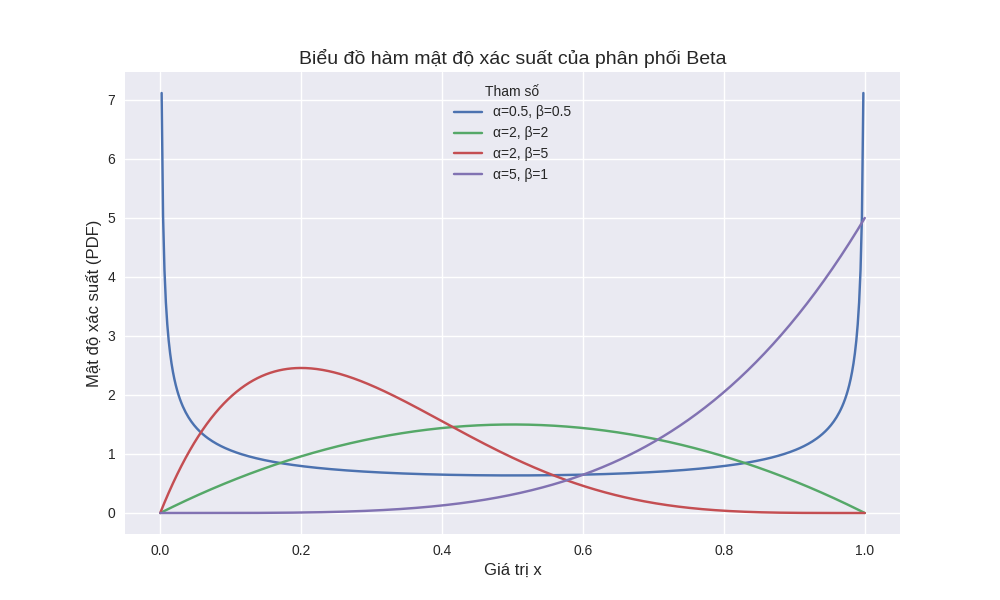
\includegraphics[width=0.7\textwidth]{images/Beta Distribution-PDF.png} % Placeholder cho hình ảnh
		\caption{Hàm mật độ xác suất của Phân phối Beta với các tham số khác nhau.}
		\label{fig:Beta Distribution-PDF}
	\end{figure}
\newpage	
	\begin{figure}[h!]
		\centering
		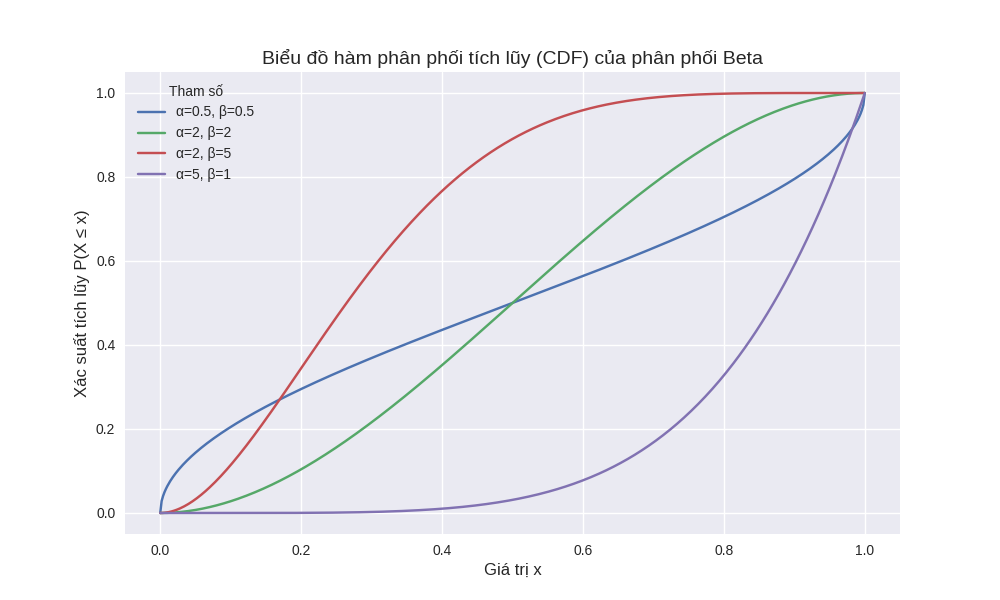
\includegraphics[width=0.7\textwidth]{images/Beta Distribution-CDF.png} % Placeholder cho hình ảnh
		\caption{Hàm xác suất tích lũy của Phân phối Beta với các tham số khác nhau.}
		\label{fig:Beta Distribution-CDF}
	\end{figure}
	

\subsection{Cơ sở toán học: Phân phối Tiên nghiệm Liên hợp}

Phân phối Beta ($\text{Beta}(\alpha, \beta)$) là một phân phối xác suất liên tục được định nghĩa trên khoảng $[0, 1]$. Nó được sử dụng lý tưởng để mô hình hóa các biến ngẫu nhiên là tỷ lệ hoặc xác suất.

Trong thống kê Bayes, Phân phối Beta là tiên nghiệm liên hợp (conjugate prior) cho tham số xác suất thành công $p$ của Phân phối Nhị thức (Binomial Distribution).

\begin{itemize}
    \item \textbf{phân phối Tiên nghiệm (Prior):} Biểu thị niềm tin ban đầu của chúng ta về $p$ trước khi quan sát dữ liệu.
    \[
    p \sim \text{Beta}(\alpha, \beta)
    \]
    \item \textbf{Khả năng (Likelihood):} Mô hình hóa dữ liệu quan sát được (số lần thành công $k$ trong $n$ thử nghiệm).
    \[
    \text{Data} \mid p \sim \text{Binomial}(n, p) \quad \text{với} \quad P(k \mid p) \propto p^k (1-p)^{n-k}
    \]
    \item \text{Phân phối Hậu nghiệm (Posterior):} Phân phối sau khi cập nhật tiên nghiệm bằng dữ liệu. Nhờ tính chất tiên nghiệm liên hợp, hậu nghiệm cũng là một phân phối Beta với các tham số cập nhật.
    \[
    p \mid \text{Data} \sim \text{Beta}(\alpha', \beta')
    \]
\end{itemize}

Công thức Cập nhật Hậu nghiệm:
Nếu $\text{Prior} \sim \text{Beta}(\alpha, \beta)$ và ta quan sát $k$ thành công và $n-k$ thất bại, thì:
\[
\alpha' = \alpha + k \quad \text{và} \quad \beta' = \beta + (n-k)
\]

\subsection{Ví dụ thực tế: Ước lượng Tỷ lệ Phiếu ủng hộ}

Bài toán: Ước lượng xác suất $p$ (tỷ lệ cử tri ủng hộ ứng cử viên A trong một quần thể).

\textbf{Thiết lập Tiên nghiệm:}
Chúng ta chọn tiên nghiệm $\text{Beta}(1, 1)$, được biết đến là tiên nghiệm đồng nhất (Uniform Prior), vì nó gán xác suất như nhau cho mọi giá trị của $p$ trong khoảng $[0, 1]$, thể hiện sự thiếu thông tin ban đầu.

\[
p \sim \text{Beta}(1, 1) \quad (\text{với } \alpha=1, \beta=1)
\]

\textbf{Dữ liệu Quan sát (Observation):}
Chúng ta thực hiện một cuộc thăm dò với $n=20$ người, thu được:
\begin{itemize}
    \item Số lần thành công (ủng hộ): $k = 12$
    \item Số lần thất bại (không ủng hộ): $n-k = 8$
\end{itemize}
\newpage
\textbf{Tính toán Phân phối Hậu nghiệm:}
Áp dụng công thức cập nhật hậu nghiệm:
\begin{itemize}
    \item $\alpha' = \alpha + k = 1 + 12 = 13$
    \item $\beta' = \beta + (n-k) = 1 + 8 = 9$
\end{itemize}

Phân phối hậu nghiệm cho $p$ là:
\[
p \mid \text{Data} \sim \text{Beta}(13, 9)
\]

Kết luận: 
Phân phối $\text{Beta}(13, 9)$ là phân phối hậu nghiệm, 
biểu diễn sự không chắc chắn của chúng ta về tỷ lệ ủng hộ $p$ sau khi đã xem xét dữ liệu thăm dò. Giá trị kỳ vọng (mean) của phân phối này là $\frac{\alpha'}{\alpha' + \beta'} = \frac{13}{13+9} \approx 0.59$, cho thấy tỷ lệ ủng hộ có khả năng cao là khoảng $59\%$.
\section{Phân phối Dirichlet (Dirichlet Distribution)}
	Phân phối Dirichlet là một phân phối xác suất đa biến liên tục trên một simplex tiêu chuẩn. Nó là tổng quát hóa của phân phối Beta cho nhiều hơn hai danh mục và thường được sử dụng làm phân phối tiên nghiệm cho các tham số của phân phối Categorical hoặc phân phối đa thức (multinomial distribution).
	
	\subsection{Định nghĩa}
		Một vector ngẫu nhiên $X = (X_1, X_2, \dots, X_K)$ tuân theo phân phối Dirichlet với tham số vector $\boldsymbol{\alpha} = (\alpha_1, \alpha_2, \dots, \alpha_K)$ với $\alpha_i > 0$ cho mọi $i$, ký hiệu $X \sim \text{Dirichlet}(\boldsymbol{\alpha})$, có hàm mật độ xác suất được cho bởi:
		\[ f(x_1, \dots, x_K; \alpha_1, \dots, \alpha_K) = \frac{1}{B(\boldsymbol{\alpha})} \prod_{i=1}^K x_i^{\alpha_i-1} \]
		với $x_i > 0$, $\sum_{i=1}^K x_i = 1$.
		
		Trong đó, $B(\boldsymbol{\alpha})$ là hàm Beta đa biến (multivariate beta function), được định nghĩa là:
		\[ B(\boldsymbol{\alpha}) = \frac{\prod_{i=1}^K \Gamma(\alpha_i)}{\Gamma\left(\sum_{i=1}^K \alpha_i\right)} \]
	
	\subsection{Hàm xác suất tích lũy (Cumulative Distribution Function - CDF)}
	Hàm xác suất tích lũy của phân phối Dirichlet không có dạng đóng đơn giản và phức tạp hơn nhiều so với các phân phối một biến. Thường không được sử dụng trực tiếp.
	
	\subsection{Các đặc trưng thống kê}
	\begin{itemize}
		\item \textbf{Miền giá trị:} Simplex tiêu chuẩn 
		\[
		S_K = \left\{ (x_1, \dots, x_K) \mid x_i > 0,\; \sum_{i=1}^K x_i = 1 \right\}.
		\]

		\item \textbf{Giá trị kỳ vọng (Mean):} Đối với từng thành phần $X_i$:
		\[
		E[X_i] = \frac{\alpha_i}{\sum_{j=1}^K \alpha_j}.
		\]

		\item \textbf{Phương sai (Variance):} Đối với từng thành phần $X_i$:
		\[
		\mathrm{Var}[X_i] = 
		\frac{\alpha_i \left( \sum_{j=1}^K \alpha_j - \alpha_i \right)}
			{\left( \sum_{j=1}^K \alpha_j \right)^2 \left( \sum_{j=1}^K \alpha_j + 1 \right)}.
		\]

		\item \textbf{Mode:} Đối với từng thành phần $X_i$:
		\[
		\mathrm{Mode}_i = \frac{\alpha_i - 1}{\sum_{j=1}^K \alpha_j - K},
		\quad \text{nếu tất cả } \alpha_i > 1.
		\]

		\item \textbf{Median:} Không có dạng đóng.

		\item \textbf{Tính chất:} Phân phối Dirichlet là liên hợp tiên nghiệm cho phân phối Categorical và phân phối Đa thức.
	\end{itemize}

	
	\subsection{Biểu đồ minh họa}
	Việc minh họa hàm	 mật độ xác suất của phân phối Dirichlet yêu cầu các biểu đồ trên simplex. Đối với $K=3$, chúng ta có thể sử dụng biểu đồ tam giác.
	
	\begin{figure}[h!]
		\centering
		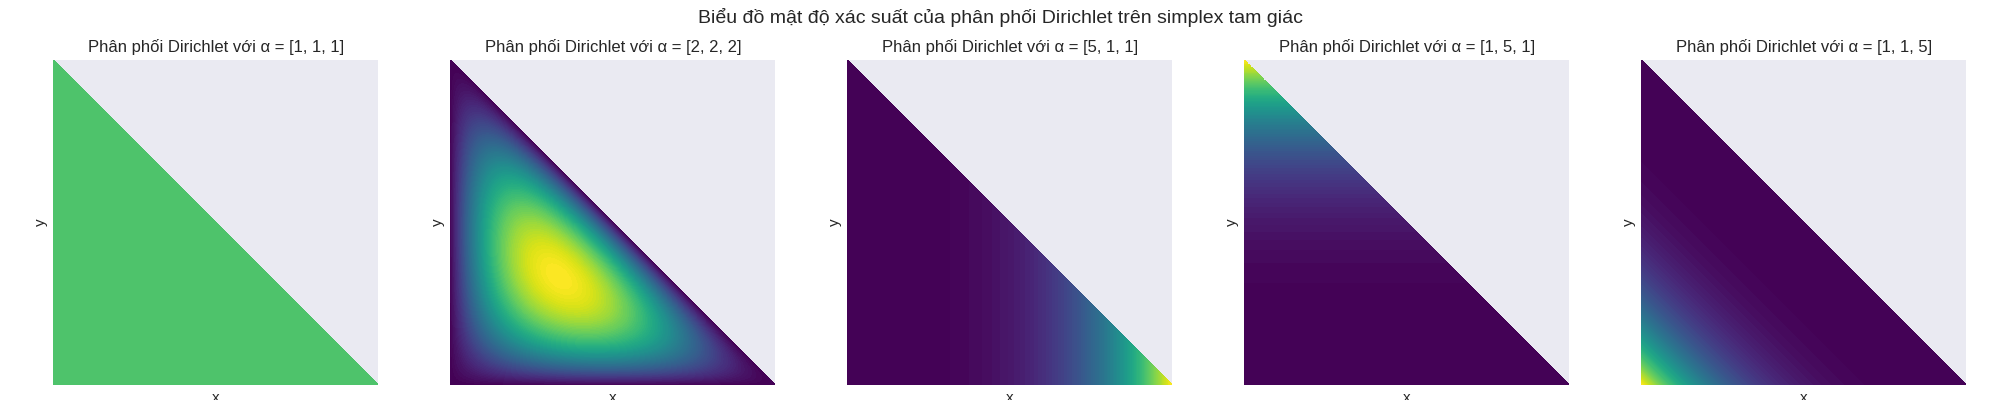
\includegraphics[width=0.7\textwidth]{images/Dirichlet Distribution-PDF.png} % Placeholder cho hình ảnh
		\caption{Hàm mật độ xác suất của Phân phối Dirichlet với $K=3$ và các tham số khác nhau.}
		\label{fig:pngDirichlet Distribution-PDF}
	\end{figure}
	
	Biểu đồ minh hoạt hàm xuất sắc tích lũy của phân phối Dirichlet
	
	\begin{figure}[h!]
		\centering
		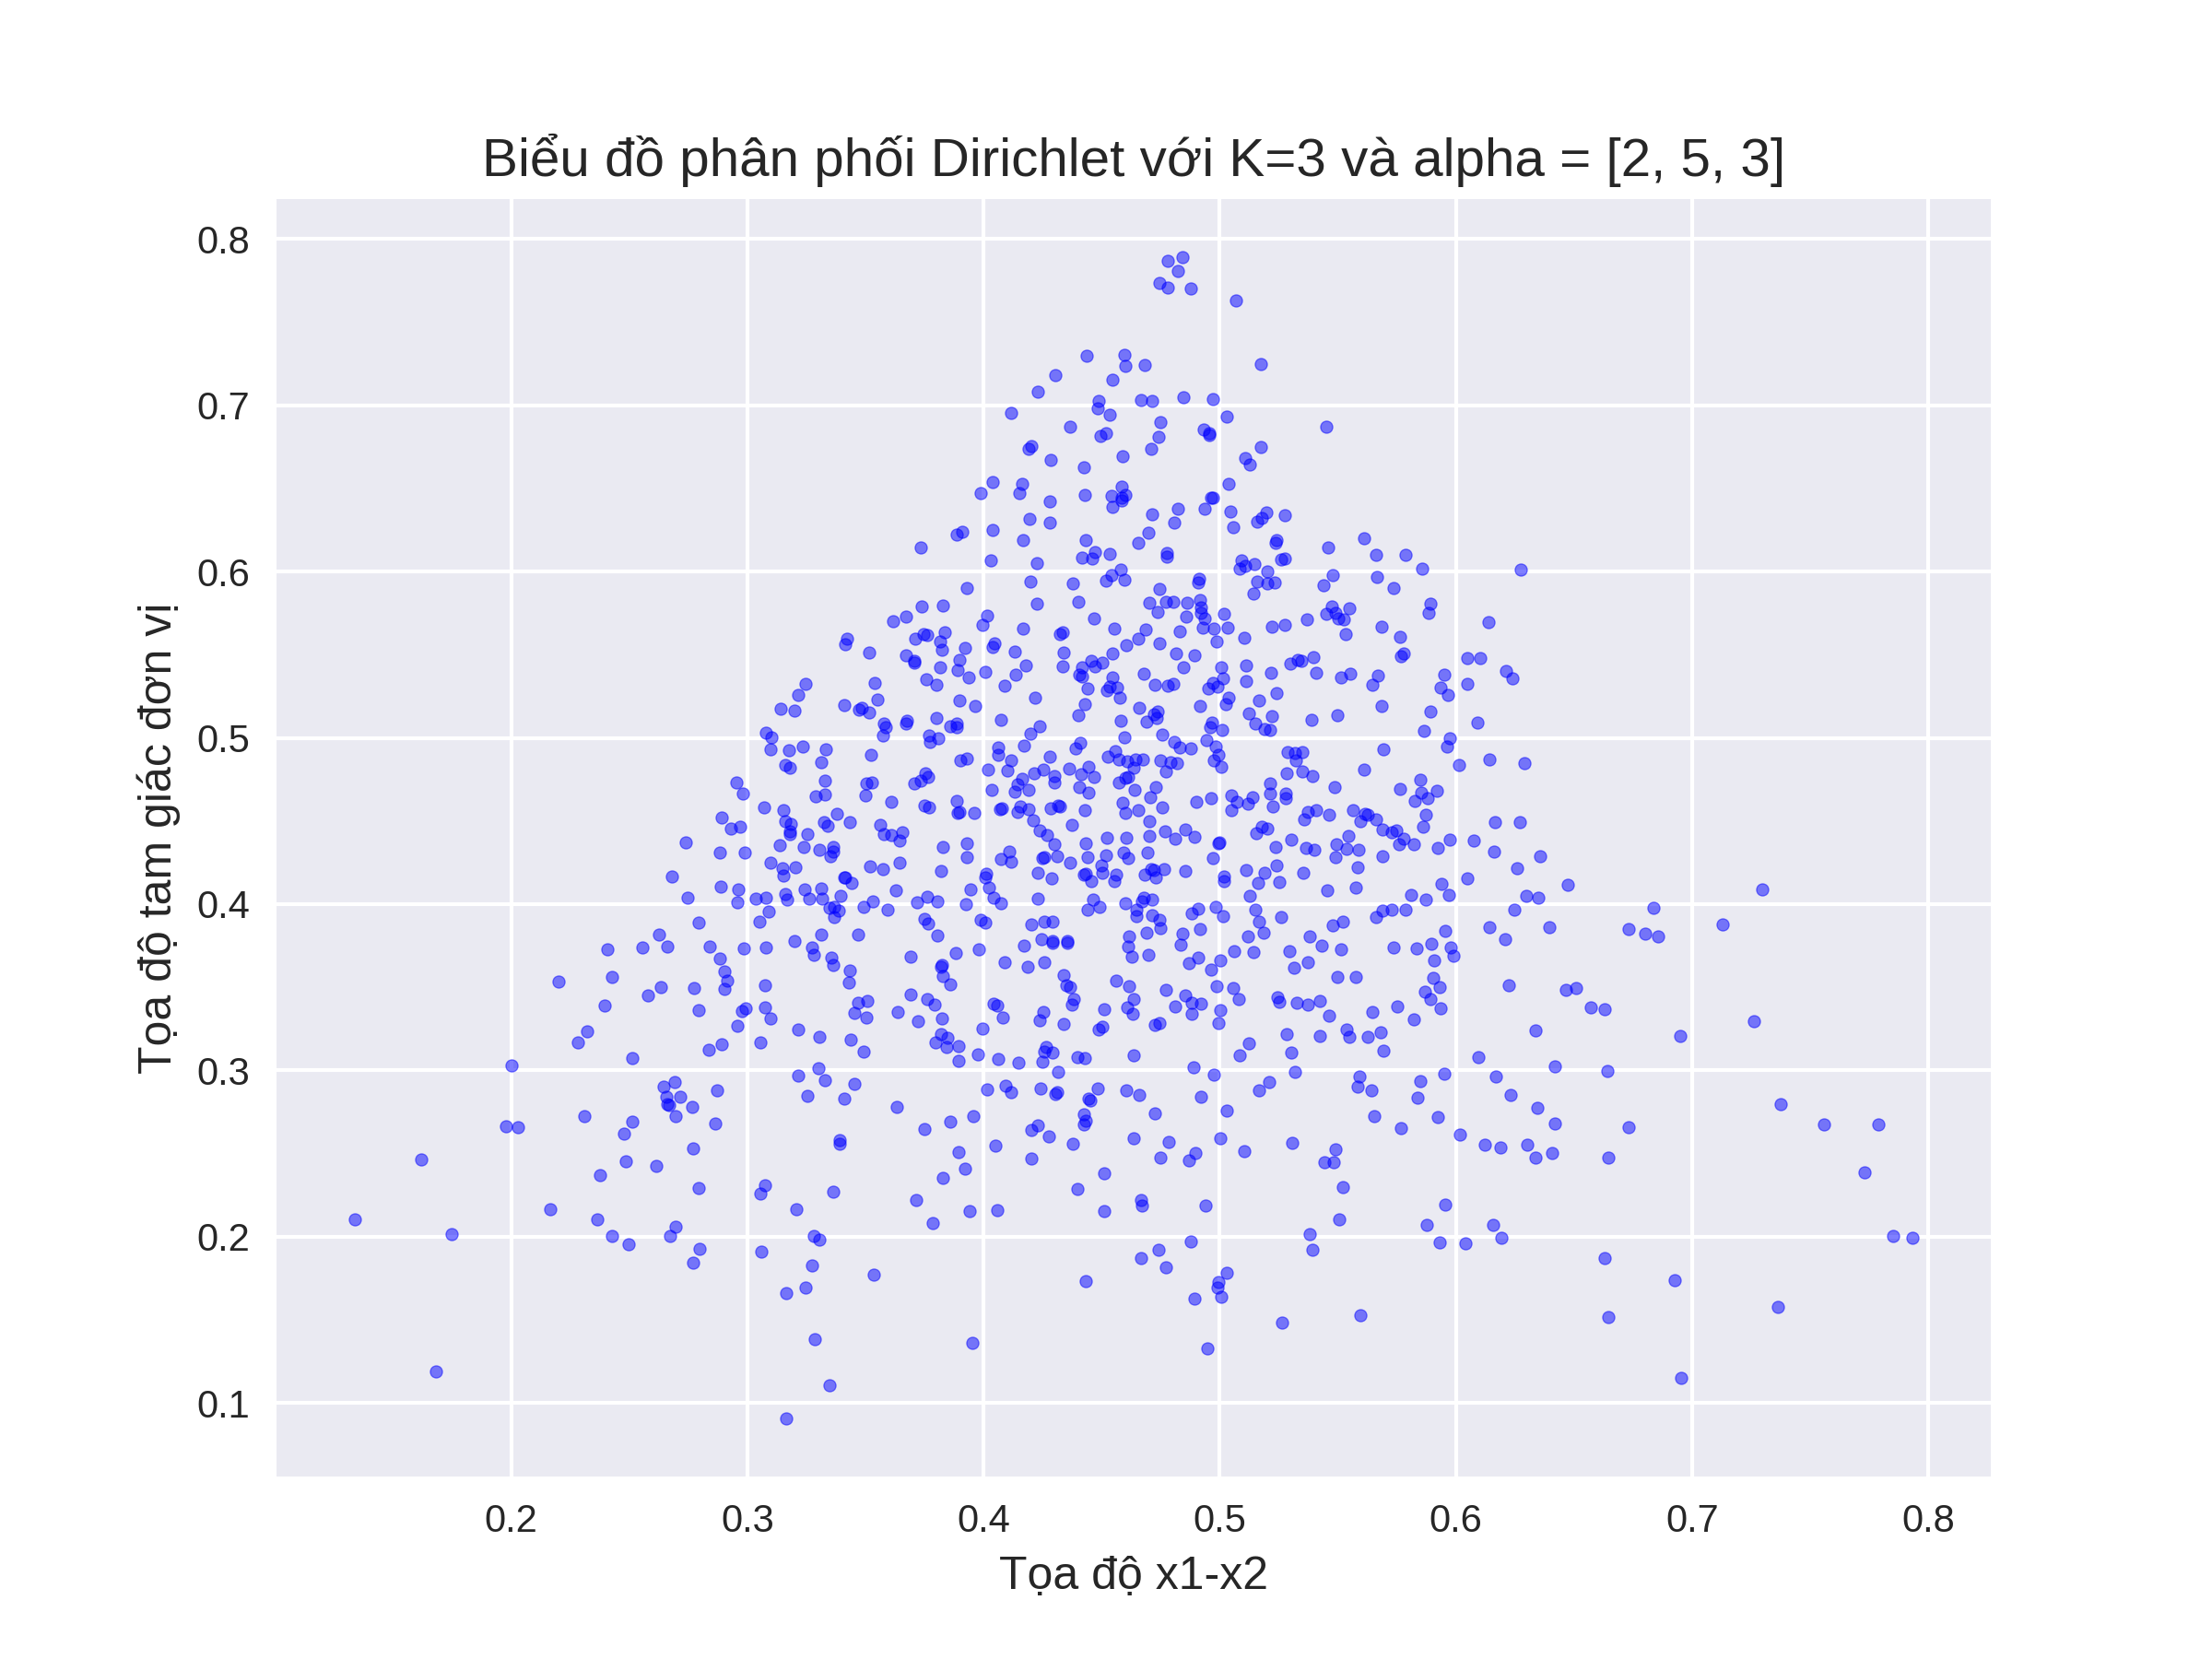
\includegraphics[width=0.7\textwidth]{images/Dirichlet Distribution-CDF.png} % Placeholder cho hình ảnh
		\caption{Hàm mật độ xác suất của Phân phối Dirichlet với $K=3$ và các tham số khác nhau.}
		\label{fig:pngDirichlet Distribution-CDF}
	\end{figure}
	
	\subsection{Ví dụ dữ liệu và bài toán thực tế}
		Phân phối tiên nghiệm cho phân loại văn bản
		Trong mô hình hóa chủ đề (topic modeling) như Latent Dirichlet Allocation (LDA), 
		phân phối Dirichlet được sử dụng làm phân phối tiên nghiệm cho hai cấp độ:
		\begin{itemize}
			\item Phân phối các chủ đề trên một tài liệu (document-topic distribution).
			\item Phân phối các từ trên một chủ đề (topic-word distribution).
		\end{itemize}
		Ví dụ, $\text{Dirichlet}(\boldsymbol{\alpha})$ với $\alpha_i$ nhỏ (ví dụ, $\alpha_i=0.1$) sẽ khuyến khích các phân phối thưa, nghĩa là mỗi tài liệu có xu hướng chỉ nói về một vài chủ đề chính.
	
		Phân phối tiên nghiệm cho xác suất đa thức
		Giả sử chúng ta có một thí nghiệm với $K$ kết quả có thể xảy ra, mỗi kết quả có xác suất $p_i$. Vector $(p_1, \dots, p_K)$ với $\sum p_i = 1$ có thể được mô hình hóa bằng phân phối Dirichlet. Ví dụ, tỷ lệ các loại sản phẩm khác nhau được bán trong một siêu thị.
